% METHOD OF AVERAGING
\chapter{Method of averaging}
Following \href{https://www.phys.uconn.edu/~rozman/Courses/P2400_17S/downloads/averaging.pdf}{Rozman}, we consider the second order non-linear differential equation
\begin{gather}\label{eqn:moa-gen-form}
	\frac{\md^2 x}{\md t^2} + \epsilon \left(\frac{\md x}{\md t}\right)^3 + x = 0, \qquad \epsilon > 0
\end{gather}
with the initial conditions
\begin{gather}
	x(0) = 1	\qquad \dot{x}(0) = 0
\end{gather}
The equation describes a nonlinear oscillator with the `friction force' proportional to the third power of the velocity. Multiply eqn. \ref{eqn:moa-gen-form} with $\dot{x}$ to write
\begin{gather*}
	\frac{\md}{\md t} \left(\frac{1}{2} \dot{x}^2 + \frac{1}{2}x^2\right) = -\epsilon \dot{x}^4
\end{gather*}
where the term inside the parenthesis is the mechanical energy of the oscillator $E(t) \ge 0$ with $E(0)=1/2$. Clearly this energy decays, the rate of which is controlled by the parameter $\epsilon$.
\section*{Numerical solution}
It is always instructive to first study the numerical solution to the problem. This is achieved by rewriting the equation as a system of two coupled first order differential equations
\begin{align*}
	\frac{\md x}{\md t} &= y \\
	\frac{\md y}{\md t} &= -\epsilon y^3 - x
\end{align*}
with appropriate intial conditions. The solution is plotted in Fig. \ref{fig:nonlin-oscillator} for $\epsilon = 0.2$.
\begin{figure}[!h]
	\centering
	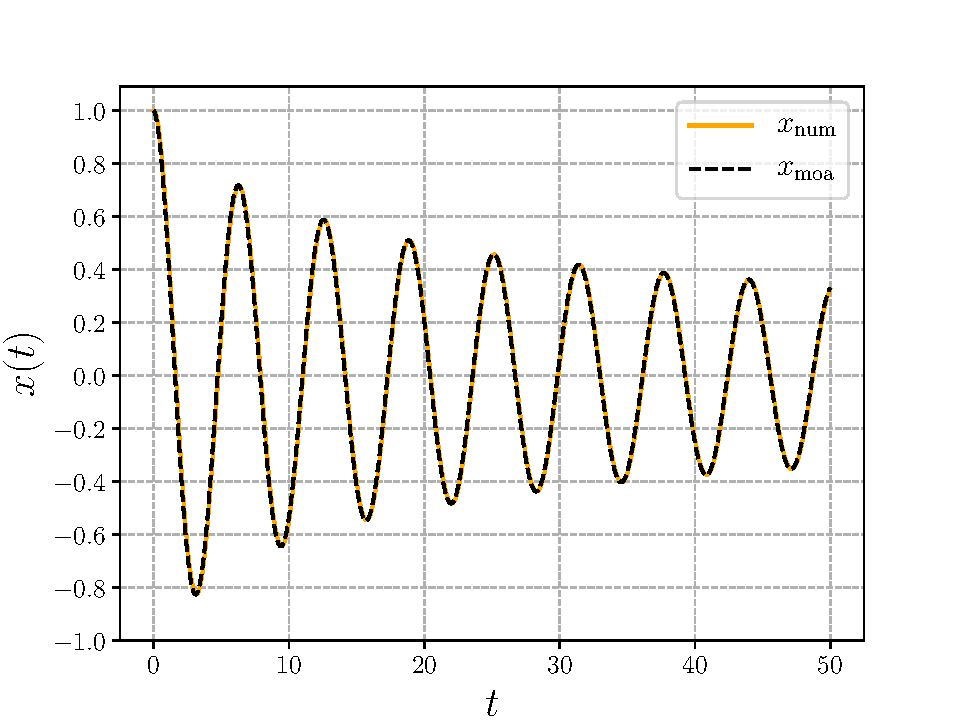
\includegraphics[width=0.7\textwidth]{./plots/pdf/nonlin-oscillator.pdf}
	\caption{ Numerical solution to eqn. \ref{eqn:moa-gen-form} and analytical approximation eqn. \ref{eqn:moa-ana-soln}. Code available through \href{https://bitbucket.org/arkabokshi/mynotes/src/master/MathematicalDoodles/nonlin-oscillator.py}{Bitbucket}.}
	\label{fig:nonlin-oscillator}
\end{figure}
Again a standard perturbative approach yields a secular term. To obtain an approximate analytic solution, we use the \emph{method of averaging}.
\section*{Analytical solution}
This approach is applicable to equations of the general form
\begin{gather}\label{eqn:moa-gen-form-2}
	\frac{\md^2 x}{\md t^2} + x = \epsilon F \left(x,\frac{\md x}{\md t}\right) ,
\end{gather}
where in our case
\begin{gather*}
	F = -\left(\frac{\md x}{\md t}\right)^3
\end{gather*}
We seek a solution to eqn. \ref{eqn:moa-gen-form} of the form
\begin{gather}\label{eqn:moa-gen-soln}
	x(t) = a(t) \cos \left(t+\psi(t)\right)
\end{gather}
The motivation for this ansatz is that when $\epsilon=0$, eqn. \ref{eqn:moa-gen-form-2} has its solution of the form eqn. \ref{eqn:moa-gen-soln} with $a$ and $\psi$ constants. For small values of $\epsilon$, we expect the same form of the solution to be approximately valid, but now $a(t)$ and $\psi(t)$ are expected to slowly vary with time $t$. Differentiating eqn. \ref{eqn:moa-gen-soln}
\begin{gather*}
	\dot{a} \cos(t+\psi) - a (1+\dot{\psi}) \sin(t+\psi) = -a \sin (t+\psi) 
\end{gather*}
where in the rhs, we have assumed slow variations in $a$ and $\psi$. Therefore
\begin{gather}\label{eqn:moa-da}
	\dot{a} \cos(t+\psi) - a \dot{\psi} \sin(t+\psi) = 0
\end{gather}
With the hierarchy of equations
\begin{align*}
	x &= a \cos (t+\psi) \\
	\frac{\md x}{\md t} &= -a \sin (t+\psi) \\
	\frac{\md^2 x}{\md t^2} &= -\dot{a} \sin(t+\psi) - a (1+\dot{\psi}) \cos(t+\psi)
\end{align*}
eqn. \ref{eqn:moa-gen-form} yields
\begin{gather}\label{eqn:moa-dpsi}
	-\dot{a} \sin(t+\psi) - a \dot{\psi} \cos(t+\psi) = \epsilon a^3 \sin^3 (t+\psi)
\end{gather}
Using eqns. \ref{eqn:moa-da} and \ref{eqn:moa-dpsi} we obtain two differential equations for $\dot{a}$ and $\dot{\psi}$
\begin{align*}
	\frac{\md \psi}{\md t} &= -\epsilon a^2 \sin^3 (\phi) \cos (\phi)\\
	\frac{\md a}{\md t} &= -\epsilon a^3 \sin^4(\phi)
\end{align*}
where $\phi = t+\psi$. Now the key approximation is this:  since both $\dot{a}$ and $\dot{\psi}$ are slowly varying, we can replace them with their averages:
\begin{gather*}
	\langle \dots \rangle \equiv \frac{1}{2\pi} \int_{0}^{2 \pi} \dots \md \phi 
\end{gather*}
Using the definition of $\beta$ function (sec. \ref{sec:beta-func})
\begin{align*}
\frac{\md \psi}{\md t} &= -\epsilon a^2 \frac{1}{2\pi} \int_{0}^{2 \pi}\sin^3 (\phi) \cos (\phi) \, \md \phi = 0\\
\frac{\md a}{\md t} &= -\epsilon a^3 \frac{1}{2\pi} \int_{0}^{2\pi} \sin^4(\phi) \, \md \phi = -\epsilon a^3 \frac{1}{2\pi} 2 \beta \left(\frac{5}{2},\frac{1}{2}\right) \\
&= -\epsilon a^3 \frac{3}{8}
\end{align*}
We thereby derive
\begin{gather*}
	\psi(t) = \mathrm{const.} \\
	a(t) = \frac{1}{\sqrt{\frac{3}{4}\epsilon t + \frac{1}{a^2(0)}}} 
\end{gather*}
We choose $a(0)=1$ and $\psi(t)=0$ to match the numerical solution (Fig. \ref{fig:nonlin-oscillator}), yielding
\begin{gather}\label{eqn:moa-ana-soln}
	x(t) = \frac{\cos t}{\sqrt{\frac{3}{4}\epsilon t + 1}} \quad .
\end{gather}

\section*{Duffing oscillator revisited}\label{sec:moa-duffing}
Equation \ref{eqn:moa-da} is unchanged and only the rhs of eqn. \ref{eqn:moa-dpsi} is replaced with $-\epsilon a^3 \cos^3(t+\psi)$. The equations for $\dot{a}$ and $\dot{\psi}$ are
\begin{align*}
	\frac{\md \psi}{\md t} &= \frac{1}{2\pi} \int_{0}^{2\pi} \epsilon a^2 \cos^4 (t+\psi) \, \md t\\
	&=\frac{3}{8} \epsilon a^2 \\
	\frac{\md a}{\md t} &= \frac{1}{2\pi}\int_{0}^{2\pi}\epsilon a^3 \sin(t+\psi) \cos^3(t+\psi) \, \md t = 0
\end{align*}
where we can employ a straightforward change of variable $t+\psi = \phi$ with $\md \phi = \md t$. Applying the initial condition 
\begin{gather*}
	y(t) = \cos \left(t + 3 \epsilon t / 8\right) \quad .
\end{gather*}




